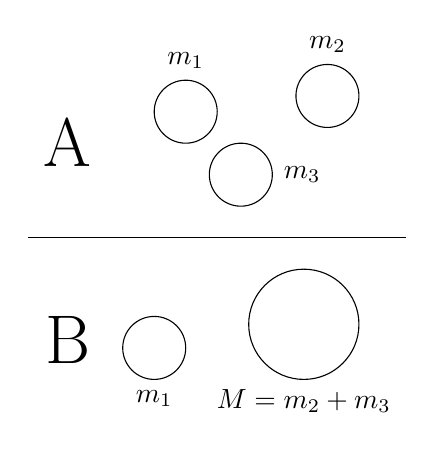
\begin{tikzpicture}
\node at (0,2.5) {\fontsize{50pt}{50pt}\selectfont A};
\node at (0,0) {\fontsize{50pt}{50pt}\selectfont B};
\draw  (1.5,2.9) circle (0.4);
\draw  (3.3,3.1) circle (0.4);
\draw  (2.2,2.1) circle (0.4);
\draw  (1.1,-0.1) circle (0.4);
\draw  (3,0.2) circle (0.7);
\node at (1.5,2.9) [above=12] {$m_1$};
\node at (3.3,3.1) [above=12] {$m_2$};
\node at (2.2,2.1) [right=12] {$m_3$};
\node at (1.1,-0.1) [below=12] {$m_1$};
\node at (3,0.2) [below=20] {$M=m_2+m_3$};
\draw (-0.5,1.3) -- (4.3,1.3);
\end{tikzpicture}